\documentclass[aspectratio=169,10pt]{beamer}
\usetheme{default}
\setbeamertemplate{navigation symbols}{}
\setbeamertemplate{footline}[frame number]
\usepackage[T1]{fontenc}
\usepackage{lmodern,booktabs}
\newcommand{\code}[1]{\texttt{#1}}
\graphicspath{{../../}}
\title{Design Patterns in a Django Food-Ordering Application}
\subtitle{23CSE455 Case Study --- Team A1 (CSE A)}
\author{Aadil Nizar \and Adil Najeem \and Athul Yesudas \and Hima C \and M Krishnapriya \and Muhammed Faais A}
\date{2026-10-11}
\begin{document}

\begin{frame}
\titlepage
\centering\footnotesize Application: HarshavardhanVemali/campus-food-ordering, commit 83998629. Full report: \code{A1\_Report.pdf}.
\end{frame}

\begin{frame}{Application and architecture}
\begin{columns}[T]
\column{0.42\textwidth}\small
\begin{itemize}
\item One Django app (\code{canteenapp}); logic mainly in function-based views (5,363 lines).
\item HTTP and WebSockets through ASGI; Channels \code{InMemoryChannelLayer}; SQLite.
\item Order-status flow: view saves order $\rightarrow$ \code{group\_send} $\rightarrow$ consumers push JSON to browsers.
\end{itemize}
\column{0.55\textwidth}
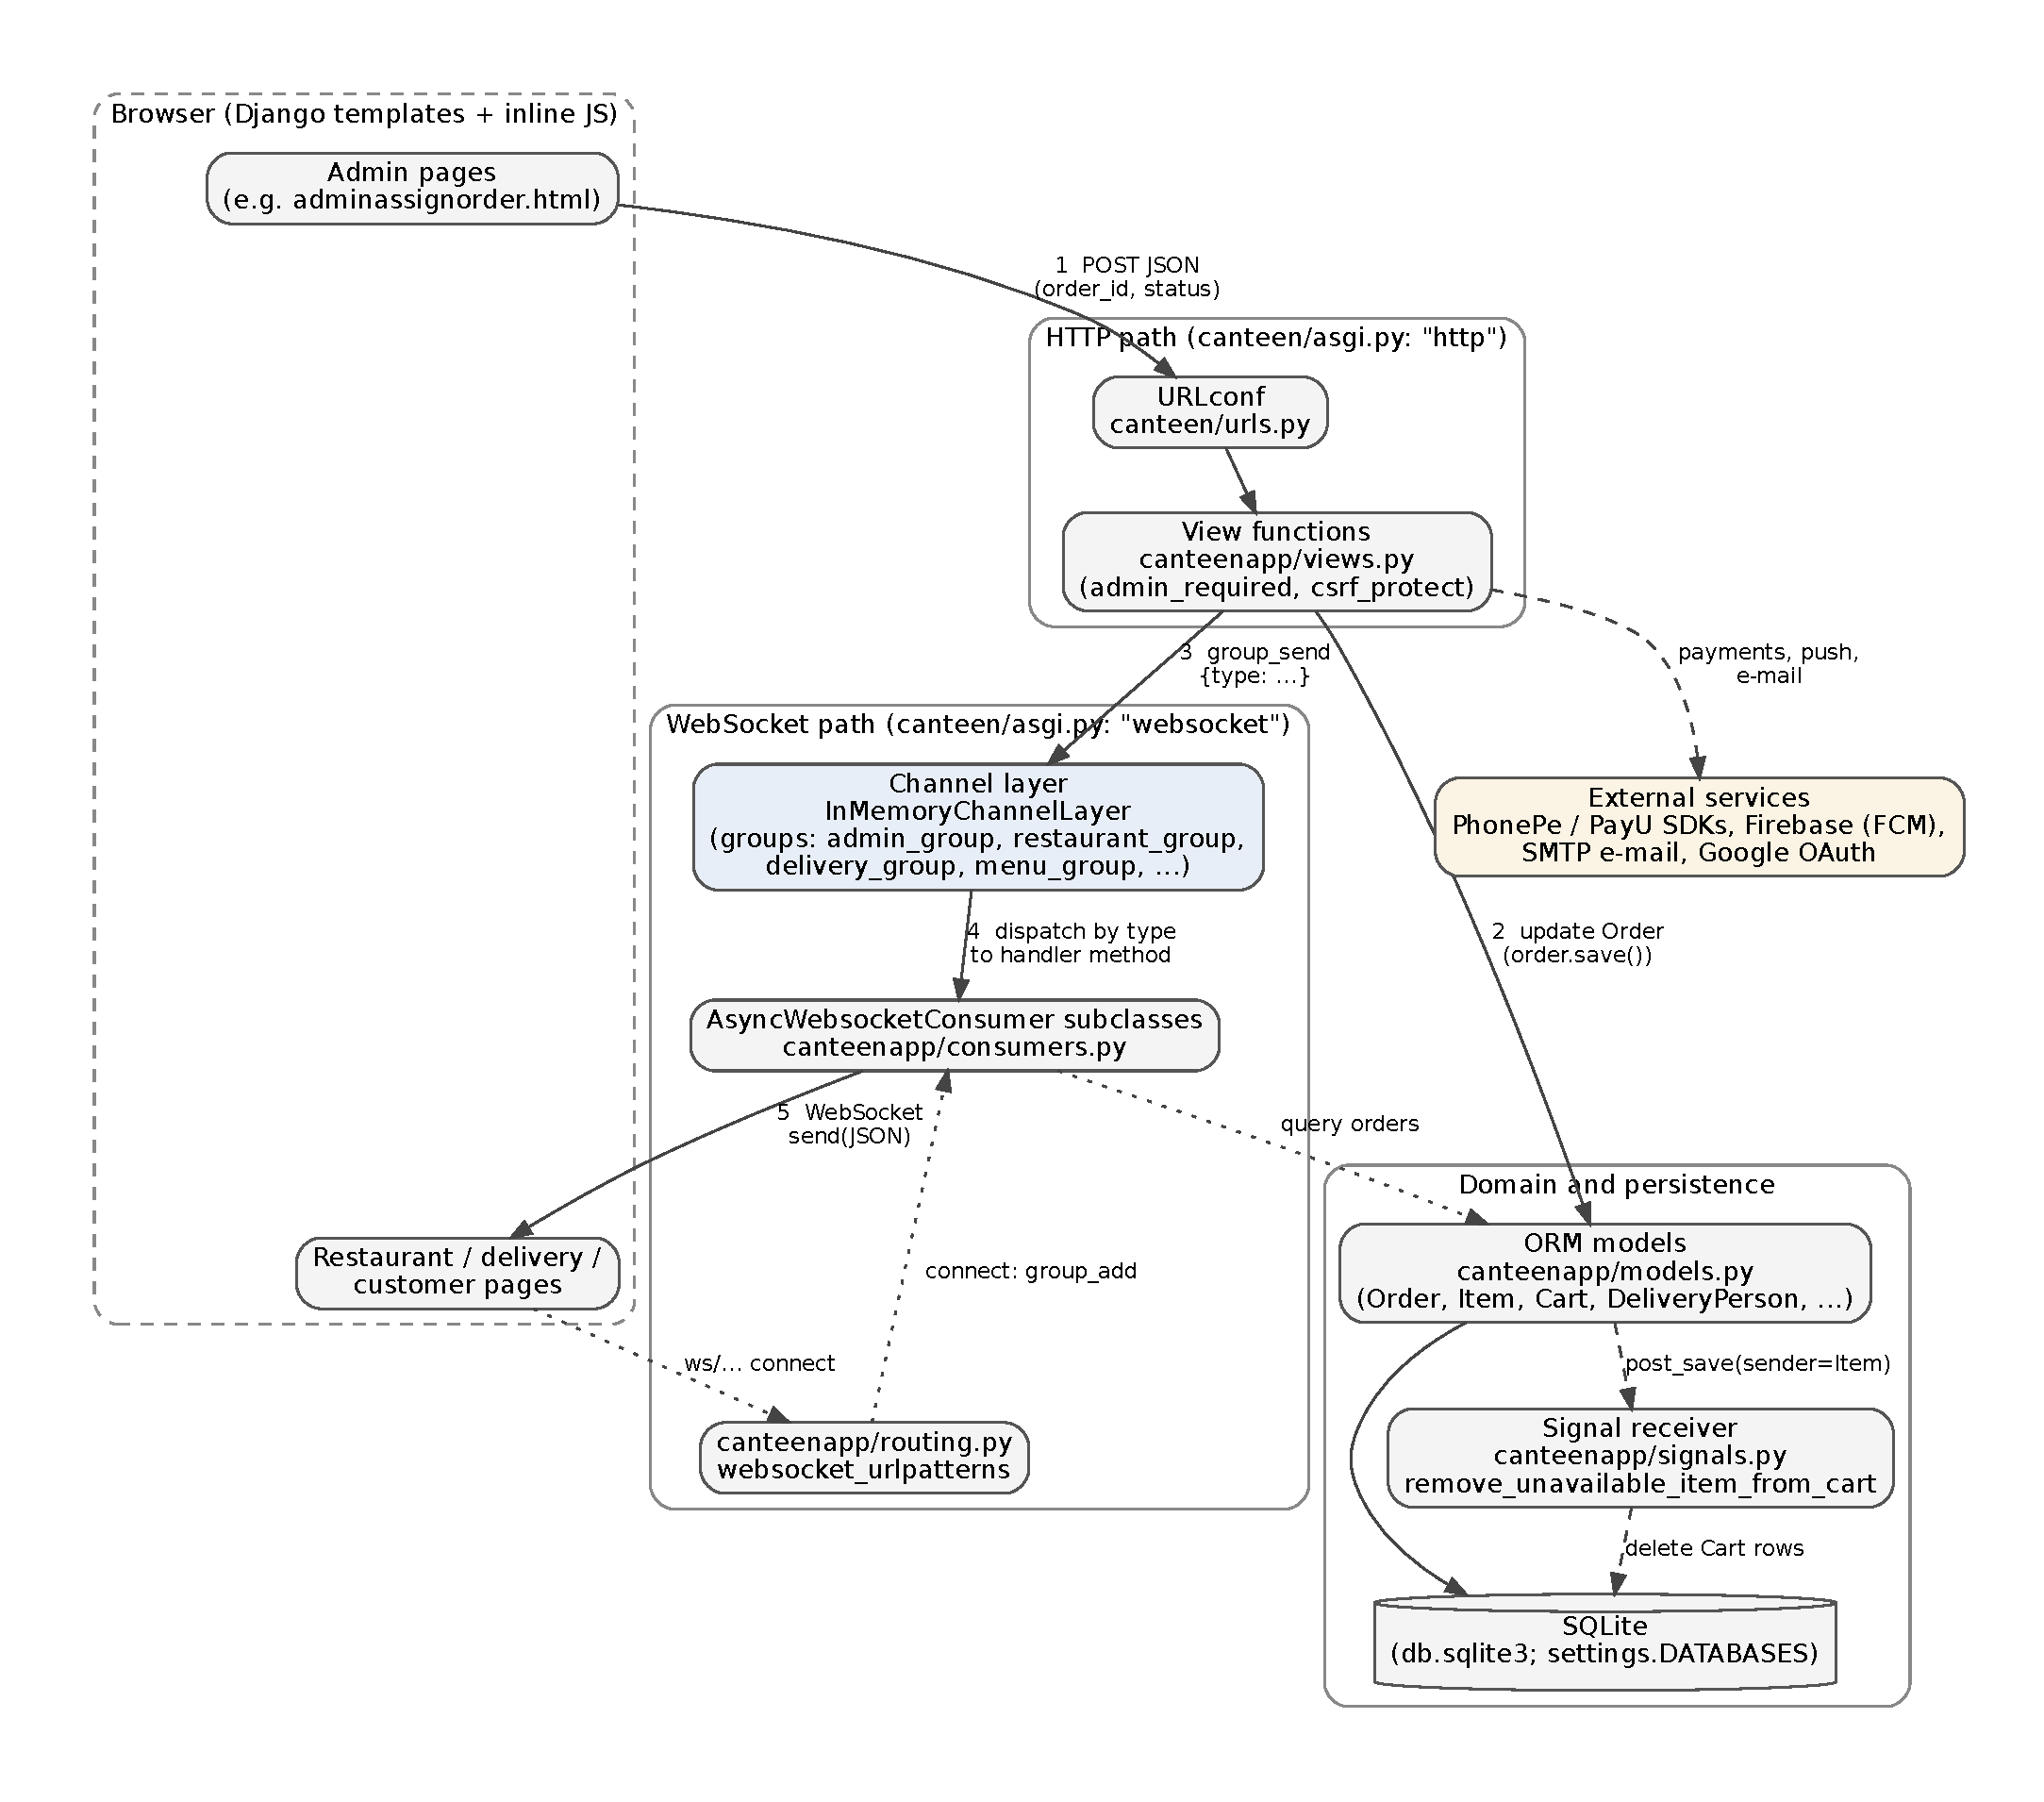
\includegraphics[width=\linewidth,height=0.78\textheight,keepaspectratio]{Part1/pattern_architecture/architecture.pdf}
\end{columns}
\end{frame}

\begin{frame}{Part 1: patterns at the baseline}
\small
\begin{tabular}{@{}lll@{}}\toprule
Instance & Pattern & Mechanism\\\midrule
Item Unavailability Cart Cleanup & Observer & \code{post\_save} signal clears carts\\
Order Status Broadcast & Observer (pub--sub) & Channels groups, 3 consumers\\\bottomrule
\end{tabular}

\vspace{1em}
\begin{itemize}
\item Totals: 1 type, 2 instances, 3 concrete classes, 13 participant symbols.
\item 12 candidates rejected (Strategy, State, Singleton, Facade, Adapter, \dots), 2 uncertain.
\item The delivery-assignment event has no live subscriber: its consumer is inside a string literal.
\end{itemize}
\end{frame}

\begin{frame}{Part 2: CH01 --- delivery-assignment policies (Strategy)}
\begin{columns}[T]
\column{0.45\textwidth}\small
\begin{itemize}
\item \code{DeliveryAssignmentPolicy} with \code{Manual} and \code{LeastWorkload} policies; \code{DeliveryAssignmentService} as context.
\item Least workload: fewest unfinished delivery orders, ties by lowest user ID.
\item 39 Django tests and 9 UI script tests pass; no migration needed.
\item Counts after CH01: 2 types, 3 instances, 5 concrete classes.
\item CH02 and CH03 were not implemented.
\end{itemize}
\column{0.53\textwidth}
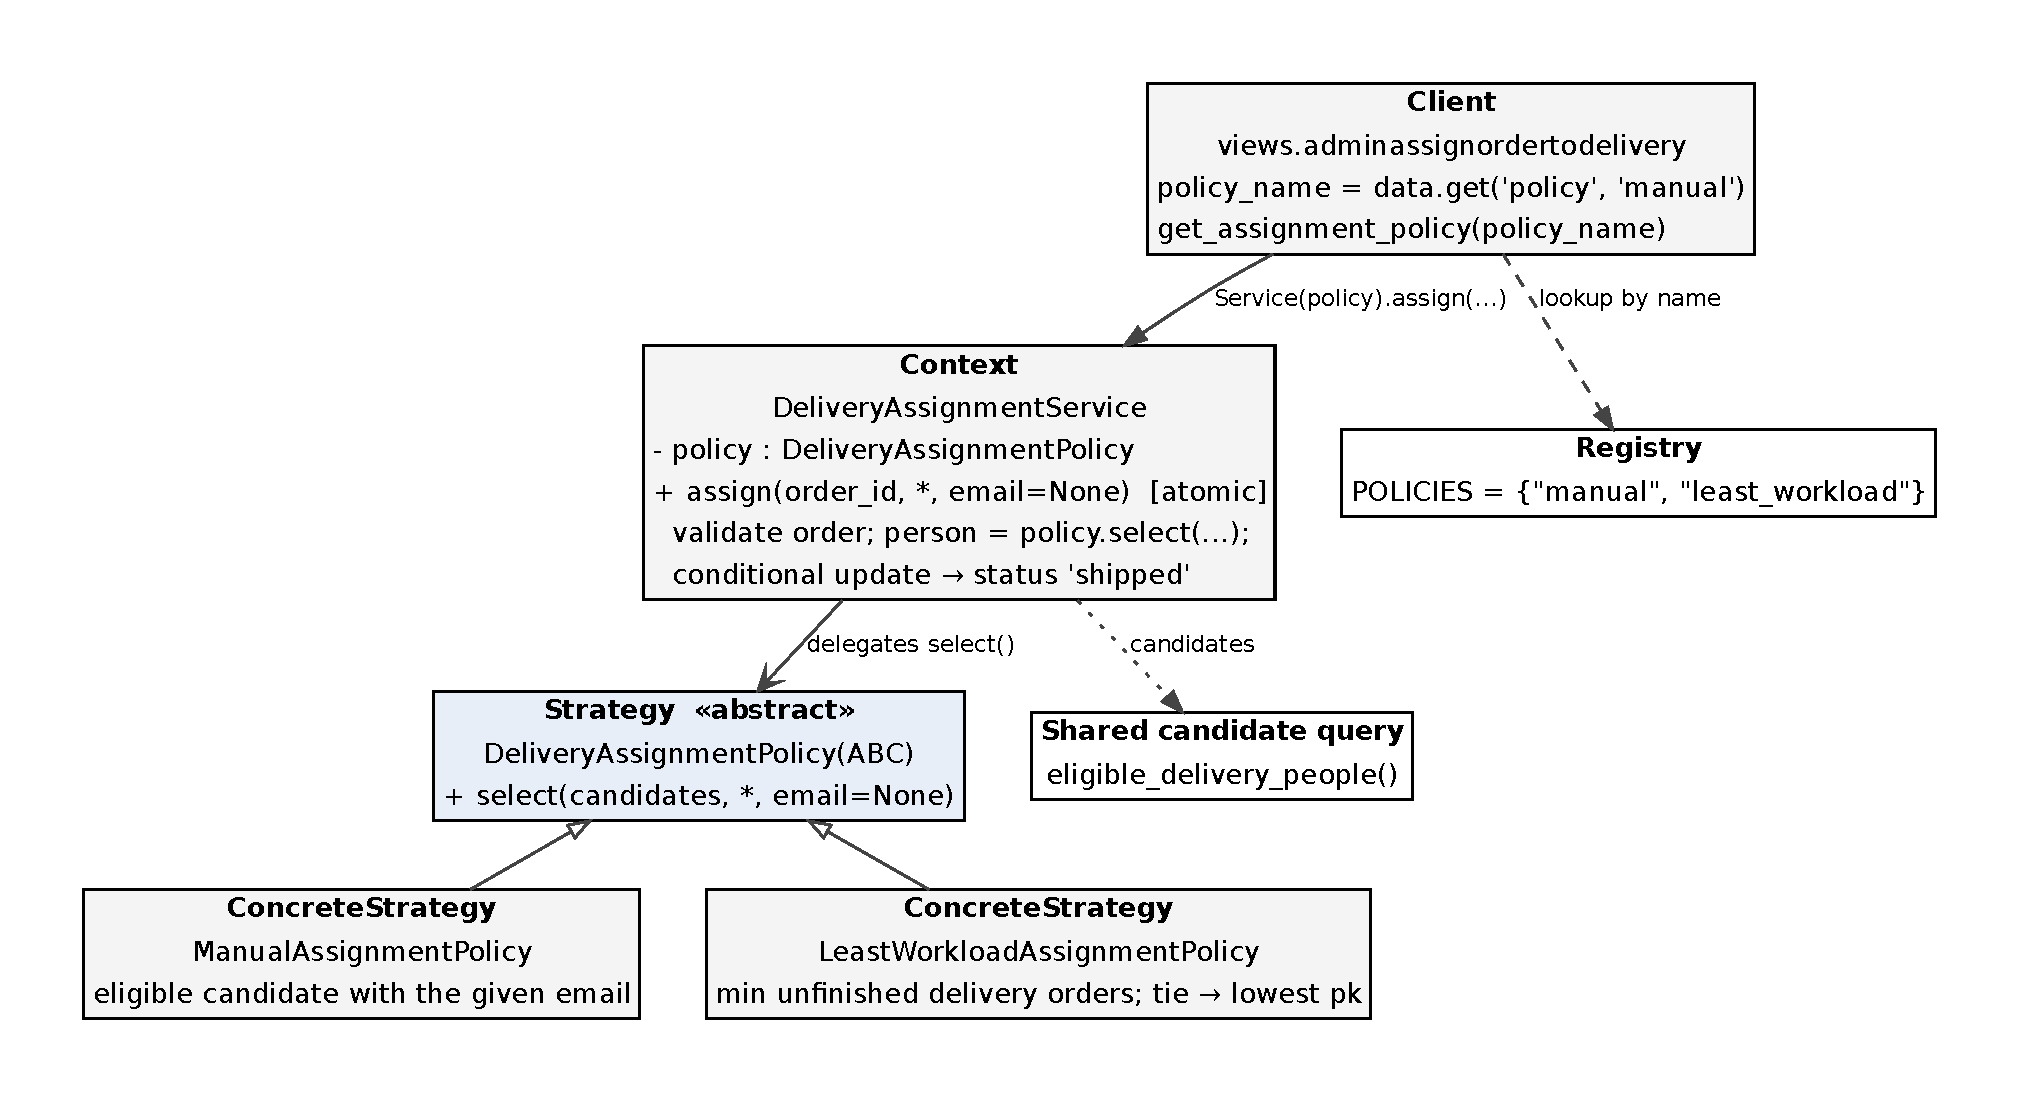
\includegraphics[width=\linewidth,height=0.75\textheight,keepaspectratio]{Part2/diagrams/strategy_delivery_assignment_CH01.pdf}
\end{columns}
\end{frame}

\begin{frame}{Part 3: cross-language comparison}
\small
\begin{tabular}{@{}lccccr@{}}\toprule
Language & Obs.\ LOC & Obs.\ CC & Str.\ LOC & Str.\ CC & Median (ms)$^\ast$\\\midrule
Java & 45 & 2 & 60 & 5 & 70.7\\
Python & 31 & 2 & 39 & 4 & 18.9\\
JavaScript & 44 & 1 & 49 & 3 & 34.7\\
C++ & 50 & 2 & 62 & 5 & 1.9\\\bottomrule
\end{tabular}

\vspace{0.6em}
\begin{itemize}
\item All four pass Observer 3/3, Strategy 2/2 and the whole-output check.
\item $^\ast$Whole-process time of the combined program (both patterns); mostly runtime start-up.
\item Java/C++ enforce the abstraction at compile time; Python/JavaScript rely on duck typing.
\end{itemize}
\end{frame}

\begin{frame}{LLM use and findings}
\small
\begin{itemize}
\item Historical analyses survive only as pasted outputs; the report-production prompts (Claude Opus 5.5, 2026-10-11) are saved in \code{data/llm/}.
\item Observer appears twice, both times through framework mechanisms rather than hand-written subjects.
\item CH01 adds a tested Strategy that keeps validation, persistence and notification in one context.
\item Baseline dependency pins conflict; the tests verify feature behaviour, not deployment readiness.
\end{itemize}
\end{frame}

\end{document}
